\documentclass[border=2pt]{standalone}
\usepackage[T1]{fontenc}
\usepackage{helvet}
\renewcommand{\familydefault}{\sfdefault}
\usepackage{amsmath,amssymb}
\usepackage{tikz}
\usetikzlibrary{positioning,arrows.meta,calc}
\definecolor{ink}{HTML}{0B0B0B}\definecolor{muted}{HTML}{52514E}
\definecolor{blue}{HTML}{2A78D6}\definecolor{lblue}{HTML}{E6EFFA}
\definecolor{orange}{HTML}{EB6834}\definecolor{lorange}{HTML}{FCE9E1}
\definecolor{aqua}{HTML}{0E8A5F}\definecolor{lgray}{HTML}{F1F0EE}
\begin{document}
\hyphenpenalty=10000\exhyphenpenalty=10000
% Two columns of 61 mm, final width about 130 mm (journal text width), so \footnotesize prints at 8 pt.
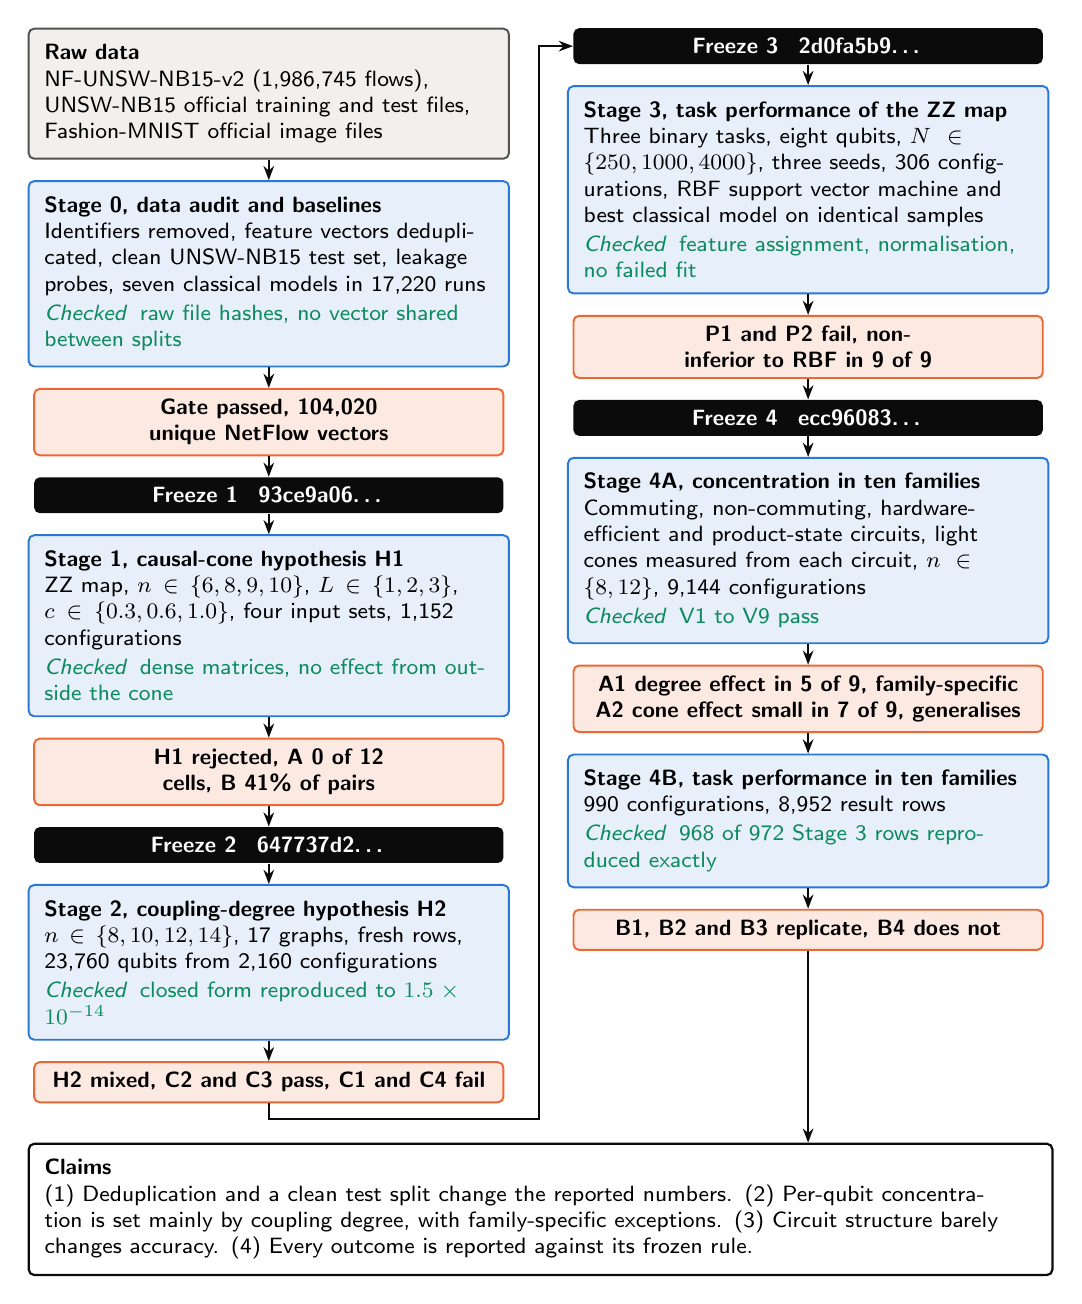
\begin{tikzpicture}[font=\footnotesize, node distance=2.6mm, >={Stealth[length=1.8mm]},
  stage/.style={draw=blue, fill=lblue, rounded corners=2pt, text width=57mm, align=left, inner sep=2mm, line width=0.7pt},
  data/.style={draw=muted, fill=lgray, rounded corners=2pt, text width=57mm, align=left, inner sep=2mm, line width=0.7pt},
  freeze/.style={fill=ink, text=white, rounded corners=2pt, text width=57mm, align=center, inner sep=1.3mm, font=\footnotesize\bfseries},
  outcome/.style={draw=orange, fill=lorange, rounded corners=2pt, text width=57mm, align=center, inner sep=1.3mm, line width=0.7pt, font=\footnotesize\bfseries},
  claim/.style={draw=ink, fill=white, rounded corners=2pt, text width=126mm, align=left, inner sep=2mm, line width=0.8pt},
  flow/.style={->, draw=ink, line width=0.7pt}]
\newcommand{\chk}[1]{\\[1pt]{\color{aqua}\textit{Checked}\enspace #1}}

% ---------------- left column
\node[data] (raw) {\textbf{Raw data}\\ NF-UNSW-NB15-v2 (1,986,745 flows), UNSW-NB15 official training and test files, Fashion-MNIST official image files};
\node[stage, below=of raw] (s0) {\textbf{Stage 0, data audit and baselines}\\ Identifiers removed, feature vectors deduplicated, clean UNSW-NB15 test set, leakage probes, seven classical models in 17,220 runs
\chk{raw file hashes, no vector shared between splits}};
\node[outcome, below=of s0] (o0) {Gate passed, 104,020 unique NetFlow vectors};
\node[freeze, below=of o0] (f1) {Freeze 1 \enspace 93ce9a06\ldots};
\node[stage, below=of f1] (s1) {\textbf{Stage 1, causal-cone hypothesis H1}\\ ZZ map, $n\in\{6,8,9,10\}$, $L\in\{1,2,3\}$, $c\in\{0.3,0.6,1.0\}$, four input sets, 1,152 configurations
\chk{dense matrices, no effect from outside the cone}};
\node[outcome, below=of s1] (o1) {H1 rejected, A 0 of 12 cells, B 41\% of pairs};
\node[freeze, below=of o1] (f2) {Freeze 2 \enspace 647737d2\ldots};
\node[stage, below=of f2] (s2) {\textbf{Stage 2, coupling-degree hypothesis H2}\\ $n\in\{8,10,12,14\}$, 17 graphs, fresh rows, 23,760 qubits from 2,160 configurations
\chk{closed form reproduced to $1.5\times10^{-14}$}};
\node[outcome, below=of s2] (o2) {H2 mixed, C2 and C3 pass, C1 and C4 fail};

% ---------------- right column
\node[freeze, right=8mm of raw.north east, anchor=north west] (f3) {Freeze 3 \enspace 2d0fa5b9\ldots};
\node[stage, below=of f3] (s3) {\textbf{Stage 3, task performance of the ZZ map}\\ Three binary tasks, eight qubits, $N\in\{250,1000,4000\}$, three seeds, 306 configurations, RBF support vector machine and best classical model on identical samples
\chk{feature assignment, normalisation, no failed fit}};
\node[outcome, below=of s3] (o3) {P1 and P2 fail, non-inferior to RBF in 9 of 9};
\node[freeze, below=of o3] (f4) {Freeze 4 \enspace ecc96083\ldots};
\node[stage, below=of f4] (s4a) {\textbf{Stage 4A, concentration in ten families}\\ Commuting, non-commuting, hardware-efficient and product-state circuits, light cones measured from each circuit, $n\in\{8,12\}$, 9,144 configurations
\chk{V1 to V9 pass}};
\node[outcome, below=of s4a] (o4a) {A1 degree effect in 5 of 9, family-specific\\ A2 cone effect small in 7 of 9, generalises};
\node[stage, below=of o4a] (s4b) {\textbf{Stage 4B, task performance in ten families}\\ 990 configurations, 8,952 result rows
\chk{968 of 972 Stage 3 rows reproduced exactly}};
\node[outcome, below=of s4b] (o4b) {B1, B2 and B3 replicate, B4 does not};

% ---------------- claims
\path let \p1=(o2.south), \p2=(o4b.south) in coordinate (low) at (0,{min(\y1,\y2)});
\node[claim, anchor=north west] (cl) at ($(raw.west |- low)+(0,-5mm)$) {\textbf{Claims}\\
(1) Deduplication and a clean test split change the reported numbers.\enspace (2) Per-qubit concentration is set mainly by coupling degree, with family-specific exceptions.\enspace (3) Circuit structure barely changes accuracy.\enspace (4) Every outcome is reported against its frozen rule.};

% ---------------- arrows
\foreach \a/\b in {raw/s0,s0/o0,o0/f1,f1/s1,s1/o1,o1/f2,f2/s2,s2/o2,f3/s3,s3/o3,o3/f4,f4/s4a,s4a/o4a,o4a/s4b,s4b/o4b}
  \draw[flow] (\a) -- (\b);
\draw[flow] (o2.south) -- ++(0,-2mm) -| ($(o2.east)!0.5!(o2.east -| f3.west)+(0,0)$) |- (f3.west);
\draw[flow] (o4b.south) -- (o4b.south |- cl.north);
\end{tikzpicture}
\end{document}
